\documentclass[border=10pt]{standalone}

\usepackage{tikz}
\usepackage{tikzsymbols}
\usetikzlibrary{calc,patterns,shapes.geometric}

\def\centerarc[#1](#2)(#3:#4:#5){\draw[#1] ($(#2)+({#5*cos(#3)},{#5*sin(#3)})$) arc (#3:#4:#5);}

\begin{document}
	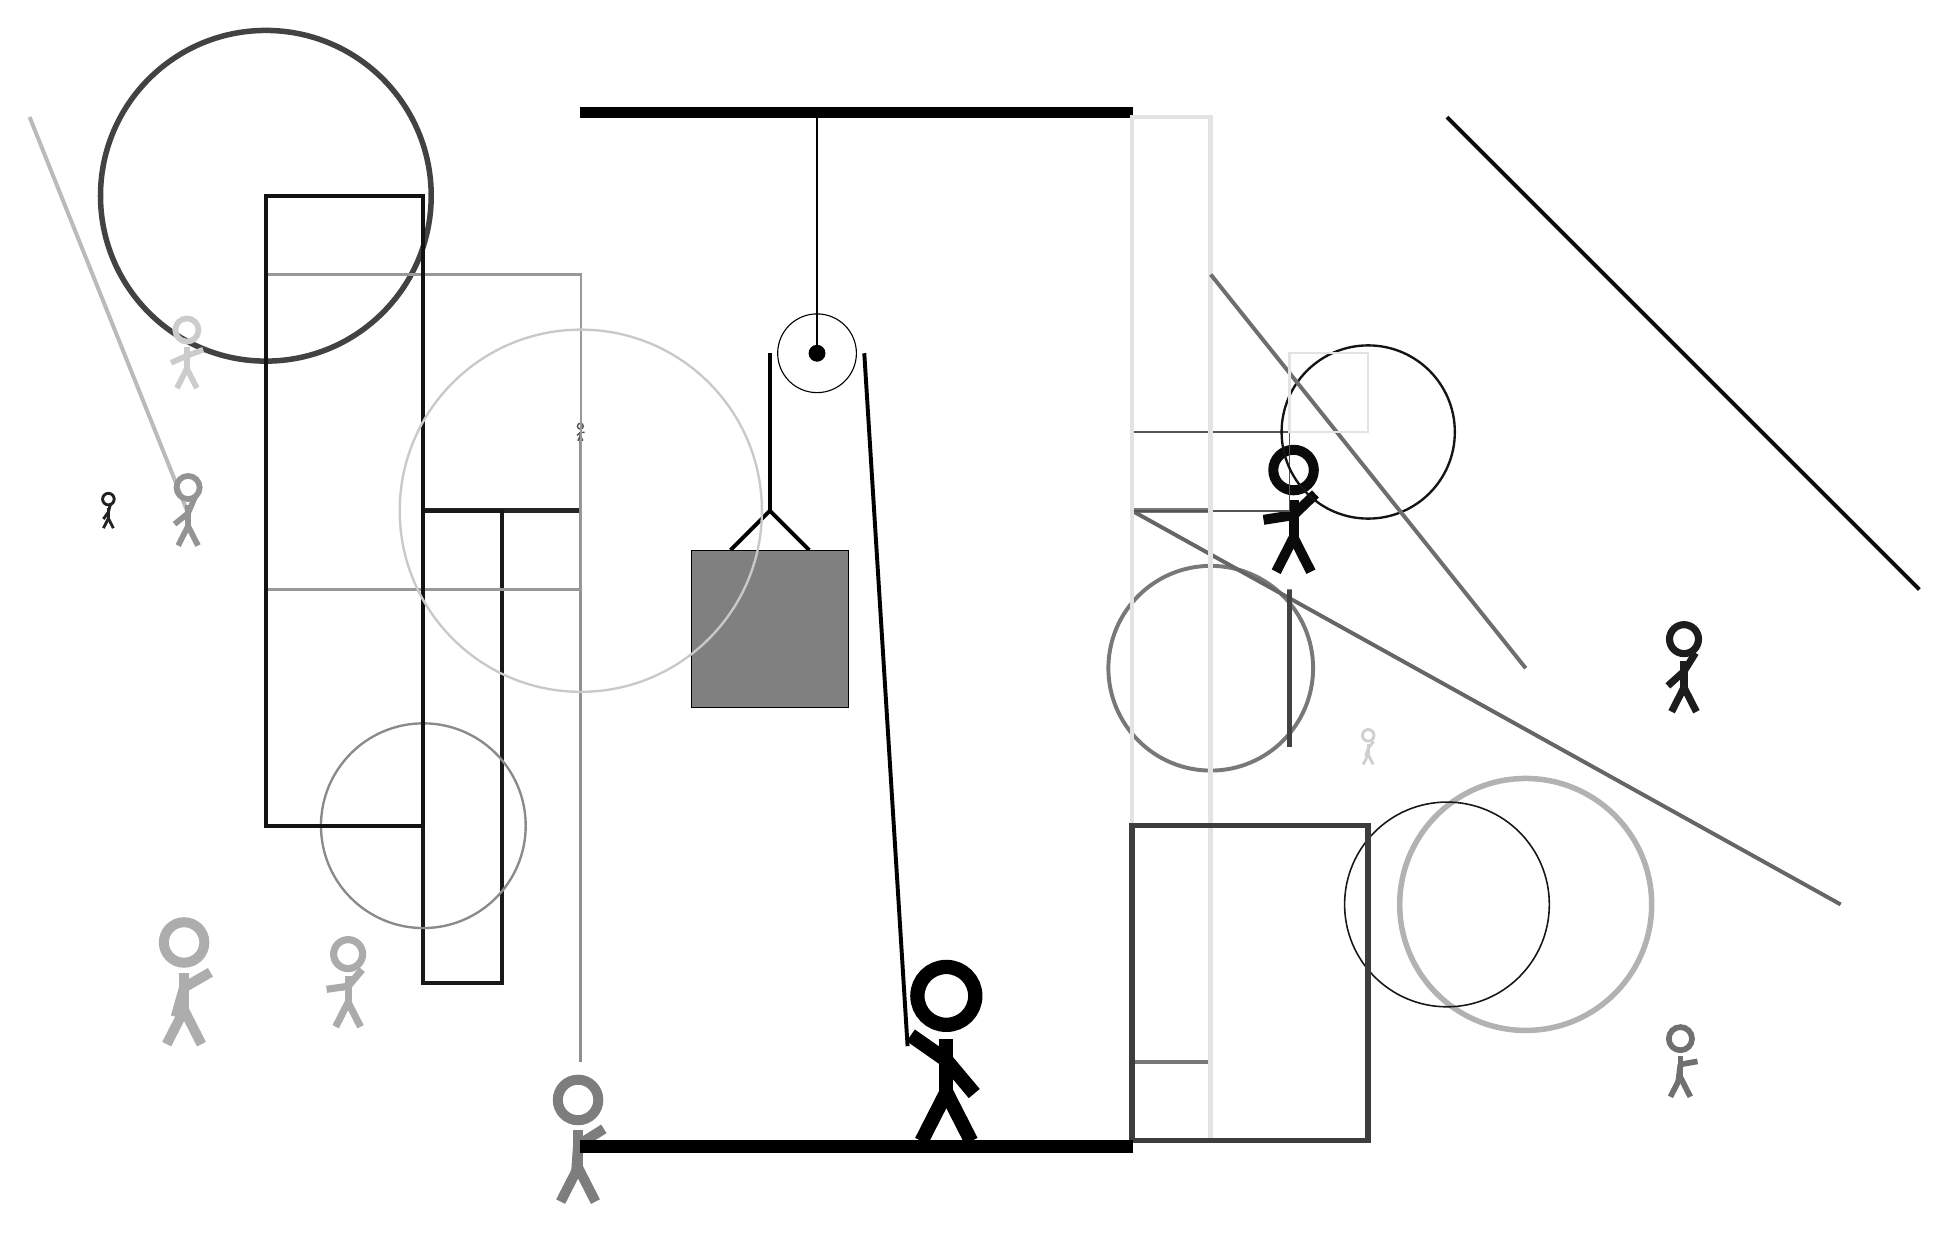
\begin{tikzpicture}
		%%%%% START %%%%%
		
		\draw[fill=black] (-2, 10) rectangle (5, 10.125);
		
		\draw (1, 7) circle (0.5);
		\draw[fill=black] (1, 7) circle (0.1);
		\draw (1, 10) -- (1, 7);
		
		\draw[line width=0.5mm] (-0.1, 4.5) -- (0.4, 5.0) -- (0.9, 4.5);
		\draw[fill=black!50] (-0.6, 4.5) rectangle (1.4, 2.5);
		
		\draw[line width=0.5mm] (0.4, 7) -- (0.4, 5.0);
		\centerarc[line width=0.5mm](1, 7)(0:180:0.6);
		\draw[line width=0.5mm](1.6, 7) -- (2.15, -1.8);
		
		\node at (2.6, -1.9) {\Strichmaxerl[10][-35][-50]};
		
		\draw[line width=0.7mm, color=black!85] (-2, 5) rectangle (-4, 5);
		
		\draw[line width=0.6mm, color=black!53] (5, 5) rectangle (6, -2);
		\draw [line width=0.5mm, color=black!53](6, 3) circle (1.3);
		\node[line width=0.7mm, color=black!56] at (12, -2) {\Strichmaxerl[4][83][10]};
		\node[line width=0.2mm, color=black!87] at (-8, 5) {\Strichmaxerl[2][55][75]};
		\draw[line width=0.5mm, color=black!60](5, 5) -- (14, 0);
		
		\draw [line width=0.5mm, color=black!50](-4, 9) circle (0.0);
		\node[line width=0.3mm, color=black!96] at (7, 5) {\Strichmaxerl[7][9][44]};
		\draw [line width=0.7mm, color=black!74](-6, 9) circle (2.1);
		\draw[line width=0.2mm, color=black!67] (5, 6) rectangle (7, 5);
		
		\draw [line width=0.7mm, color=black!30](10, 0) circle (1.6);
		\draw [line width=0.3mm, color=black!92](8, 6) circle (1.1);
		\node[line width=0.7mm, color=black!89] at (12, 3) {\Strichmaxerl[5][42][58]};
		\node[line width=0.4mm, color=black!51] at (-2, -3) {\Strichmaxerl[7][86][32]};
		\draw[line width=0.6mm, color=black!11] (5, -3) rectangle (6, 10);
		\draw[line width=0.4mm, color=black!44] (-2, 6) rectangle (-2, -2);
		\draw[line width=0.5mm, color=black!90] (-3, -1) rectangle (-4, 5);
		\draw[line width=0.5mm, color=black!27](-7, 5) -- (-9, 10);
		\node[line width=0.2mm, color=black!68] at (-2, 6) {\Strichmaxerl[1][39][4]};
		
		\draw[line width=0.6mm, color=black!76] (-3, 8) rectangle (-3, 8);
		\draw [line width=0.2mm, color=black!91](9, 0) circle (1.3);
		\node[line width=0.6mm, color=black!32] at (-7, -1) {\Strichmaxerl[7][74][30]};
		\node[line width=0.6mm, color=black!42] at (-7, 5) {\Strichmaxerl[4][39][67]};
		\node[line width=0.6mm, color=black!33] at (-5, -1) {\Strichmaxerl[5][8][50]};
		\draw[line width=0.3mm, color=black!40] (-2, 4) rectangle (-6, 8);
		
		\draw [line width=0.3mm, color=black!46](-4, 1) circle (1.3);
		\draw[line width=0.7mm, color=black!76] (5, 1) rectangle (8, -3);
		\draw[line width=0.5mm, color=black!93] (-4, 1) rectangle (-6, 9);
		
		\draw[line width=0.5mm, color=black!95](9, 10) -- (15, 4);
		
		\draw [line width=0.3mm, color=black!21](-2, 5) circle (2.3);
		\node[line width=0.3mm, color=black!19] at (8, 2) {\Strichmaxerl[2][72][51]};
		\draw[line width=0.5mm, color=black!57](10, 3) -- (6, 8);
		\node[line width=0.7mm, color=black!20] at (-7, 7) {\Strichmaxerl[4][24][20]};
		
		\draw[line width=0.6mm, color=black!74] (7, 2) rectangle (7, 4);
		
		\draw[line width=0.3mm, color=black!11] (7, 7) rectangle (8, 6);
		
		\draw[fill=black] (-2, -3) rectangle (5, -3.15);
		
		%%%%% END %%%%%
	\end{tikzpicture}
\end{document}